\section{Javascript Testing}

Nachdem eingangs verschiedene allgemeine Testarten und -methodiken aufgeführt wurden, sollen im folgenden konkrete Frameworks für die Programmiersprache Javascript aufgeführt und in Bezug auf diese allgemeinen Ansätze miteinander verglichen werden. Wie in der Einleitung erläutert, wird dabei auch untersucht, ob und wie sich die Tests in Browsern bzw. von einem eigenständigen Javascript-Interpreter ausführen lassen.

\subsection{Modultest-Frameworks}

Zunächst folgen Javascript-Frameworks, mit denen man Modultests schreiben kann.

\subsubsection{JsUnit}

\begin{figure}[H]
	\begin{center}
		
\includegraphics[width=3cm]{bilder/jsunit}
		\caption{Logo von JS-Unit}
		\label{image:jsunit}
	\end{center}
\end{figure}

JsUnit ist das Javascript-Framework der xUnit-Reihe. Es handelt sich also um eine Portierung des von Kent Beck entworfenen Modultest-Frameworks SUnit. Demzufolge bietet sie sowohl die Möglichkeit, Set-Up- und Tear-Down-Methoden, als auch Behauptungen zu formulieren:

\begin{figure}[H]
	\htmlfile{codebeispiele/jsunit.html}
	\caption{Beispiel-Datei JsUnit}
	\label{code:jsunit}
\end{figure}

Um den Test-Case auszuführen, bietet JsUnit einen Test-Runner, den man als HTML- Seite in einem beliebigen Browser öffnen kann. In diesem kann man über ein Text-Feld die oben gezeigte Test-Case-Datei referenzieren und ausführen.

\begin{figure}[H]
	\begin{center}
		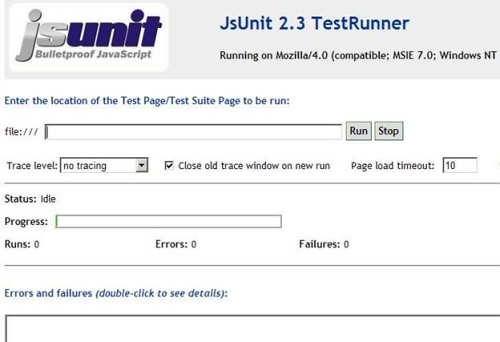
\includegraphics[width=12cm]{bilder/jsunit-testrunner}
		\caption{JS-Unit Testrunner}
		\label{image:jsunit-testrunner}
	\end{center}
\end{figure}

JsUnit bietet von Haus aus keine Möglichkeit, den Test-Case in einem Headless- Javascript-Interpreter auszuführen. Dadurch ist eine einfache, automatisierte Ausführung der Tests nicht möglich. Zudem bietet das Framework keine Möglichkeit, die Test-Cases in Test-Suiten zu organisieren. Die Entwicklung von JsUnit wurde inzwischen eingestellt \citep[Vgl.][]{Pivotal12}.

\subsubsection{YUI Test}

\begin{figure}[H]
	\begin{center}
	
\includegraphics[width=3cm]{bilder/yui}
		\caption{Logo von YUI}
		\label{image:yui}
	\end{center}
\end{figure}

YUI ist ein Framework zur Erstellung von interaktiven Webanwendungen. Teil dieses Frameworks ist die Komponente YUI-Test, mit der sich Modultests durchführen lassen:

\begin{figure}[H]
	\javascriptfile{codebeispiele/yui.js}
	\caption{Beispiel-Datei YUI}
	\label{code:yui}
\end{figure}

Wie man sehen kann, bietet YUI-Test einige Vorteile gegenüber JsUnit. Zum einen lassen sich die Tests besser beschreiben, da der Test- und der Test-Case-Name eine einfache Zeichenkette sind und keine Funktions- bzw. Dateinamen sein müssen. Es gibt außerdem die Möglichkeit, für fehlschlagende Tests eine Fehlerbeschreibung anzugeben. Die Test-Cases lassen sich zudem nach Belieben in Test-Suiten organisieren. Im Beispiel wird außerdem gezeigt, wie man die Testergebnisse z.B. als XML ausgeben kann. Der YUI-Test-Runner lässt sich also nicht nur innerhalb eines Browser sondern auch von einem Headless-Javascript-Interpreter ausführen \citep[Vgl.][]{Yahoo13}.

\subsubsection{Jasmine}

\begin{figure}[H]
	\begin{center}
		
\includegraphics[width=3cm]{bilder/jasmine}
		\caption{Logo von Jasmine}
		\label{image:jasmine}
	\end{center}
\end{figure}

Jasmine ist ein recht neues Modultest-Framework. Genau wie YUI-Test lassen sich Tests leicht beschreiben und gruppieren. Die Tests lassen sich ebenfalls sowohl in Browsern als auch in Headless-Interpretern ausführen. Im Gegensatz zu YUI bricht es aber mit der gewohnten xUnit-Syntax, um die Lesbarkeit der Tests zu erhöhen \citep[Vgl.][]{Pivotal13}:

\begin{figure}[H]
	\begin{center}
		\javascriptfile{codebeispiele/jasmine.js}
		\caption{Beispiel-Datei Jasmine}
		\label{code:jasmine}
	\end{center}
\end{figure}

\subsection{Integrationstest-Frameworks}

Da Javascript (egal ob server- und/oder clientseitig eingesetzt) vor allem zur Entwicklung von Webanwendungen verwendet wird, sind vor allem Integrationstest-Frameworks entstanden, mit denen man einfach deren Http-Schnittstelle testen kann.

\subsubsection{Phantom-JS}

\begin{figure}[H]
	\begin{center}
		
\includegraphics[width=3cm]{bilder/phantomjs}
		\caption{Logo von PhantomJS}
		\label{image:phantomjs}
	\end{center}
\end{figure}

Bei Phantom-JS handelt es sich um einen sogenannten Headless-Browser. So werden Browser genannt, die alle Funktionen eines Browsers bieten, dabei aber über keine graphische Ausgabe verfügen. Sie bieten sich also vor allem für eine programmatische Verwendung an \citep[Vgl.][]{Hidayat13}.

\begin{figure}[H]
	\begin{center}
		\javascriptfile{codebeispiele/phantomjs.js}
		\caption{Beispiel-Datei PhantomJS}
		\label{code:phantomjs}
	\end{center}
\end{figure}

Diesen Test kann man nun auf der Konsole ausführen:

\begin{figure}[H]
	\begin{center}
		\bashfile{codebeispiele/phantomjs.sh}
		\caption{Startbefehl PhantomJS}
		\label{bash:phantomjs}
	\end{center}
\end{figure}

Dadurch wird der Titel der Testseite auf der Konsole ausgegeben. Auf ähnlich einfache Weise lassen sich nun auch Links auf der Seite ausführen oder Formulare abschicken. Hierdurch lassen sich viele Aspekte einer Seite sinnvoll testen. Leider fehlt die Möglichkeit, den entsprechenden Test in verschiedenen nativen Browsern auszuführen.

\subsubsection{Selenium-Driver}

\begin{figure}[H]
	\begin{center}
		
\includegraphics[width=3cm]{bilder/selenium}
		\caption{Logo von Selenium}
		\label{image:selenium}
	\end{center}
\end{figure}

Selenium-Driver dient ebenfalls dazu, die Http-Schnittstelle einer Webanwendung zu testen. Im Gegensatz zu Phantom-JS implementiert dieses Tool aber keinen Browser sondern ist in der Lage über die sogenannte Web-Driver-Schnittstelle verschiedene native Browser "fernzusteuern". Dadurch lässt sich die Webanwendung tatsächlich in der echten Zielumgebung testen. Auf dem Entwicklungsrechner muss dafür lediglich der entsprechende Browser und ein entsprechender Treiber für Selenium-Driver installiert sein. Es gibt hierbei Treiber für Firefox, Internet Explorer, Google Chrome, Safari uvm. \citep[Vgl.][]{Selenium13}.

\begin{figure}[H]
	\begin{center}
		\javascriptfile{codebeispiele/selenium.js}
		\caption{Beispiel-Datei Selenium}
		\label{code:selenium}
	\end{center}
\end{figure}

\subsection{Test Driven Development}

Wir haben uns nun einige Frameworks, die grundsätzlich Modul- und Integrationstests mit Javascript ermöglichen. Bislang haben aber zumindest die Modultest-Frameworks noch keine Möglichkeit aufgezeigt, wie man Tests nicht nur automatisch auf der Konsole (z.B. über einen Headless-Browser) sondern auch automatisch in verschiedenen Browsern ausführen kann. Dies erforderte bislang immer das anlegen einer HTML-Datei, die man manuell in einem Browser öffnet. Hier kommen nun Tools ins Spiel, die genau diese Lücke füllen können.

\subsubsection{JsTestDriver}

JsTestDriver ist ein Java-Tool, mit dem man Modultests automatisch an Browser schicken kann, um sie ausführen zu lassen. Dazu wird zunächst mit Hilfe des Tools ein Webserver gestartet:

\begin{figure}[H]
	\begin{center}
		\bashfile{codebeispiele/jstestdriver.sh}
		\caption{Startbefehl JsTestDriver-Server}
		\label{bash:jstestdriver}
	\end{center}
\end{figure}

Nun kann man beliebige Browser über diesen Webserver einfangen, in dem man in ihnen die URL \emph{http://localhost:9876/capture} aufruft.

Anschließend legt man eine Konfigurationsdatei an, die die Webserver-Adresse und die auf ihr auszuführenden Tests definiert.

\begin{figure}[H]
	\begin{center}
		\yamlfile{codebeispiele/jstestdriver.yaml}
		\caption{Konfigurations-Datei JsTestDriver}
		\label{config:jstestdriver}
	\end{center}
\end{figure}

Die Tests können grundsätzlich mit verschiedenen Modultest-Frameworks geschrieben werden. JsTestDriver bietet die Möglichkeit, entsprechende Adapter zu schreiben. Für die gängigen Frameworks existieren diese bereits.

Zu guter Letzt startet man die eigentlichen Tests in den Browsern und lässt das Ergebnis z.B. in eine XML-Datei schreiben:

\begin{figure}[H]
	\begin{center}
		\bashfile{codebeispiele/jstestdriver2.sh}
		\caption{Startbefehl JsTestDriver-Tests}
		\label{bash:jstestdriver2}
	\end{center}
\end{figure}

Damit kann ein Entwickler nun zum Beispiel zu Beginn seines Arbeitstages einmalig bestimmte Browser auf dem JsTestDriver-Server registrieren und diese dann zum automatisierten Testen verwenden. Damit ist grundsätzlich die Möglichkeit für \ac{TDD} gegeben. Ein Punkte bleibt allerdings weiterhin offen: Jeder Test-Browser muss auf irgendeine Art und Weise vom Entwickler auf seinem JsTestDriver-Server registriert werden.

\subsubsection{Browser-Mocking}
Ein Nachteil der Browser-Fernsteuerung mit Hilfe von Selenium-Driver bzw. JsTestDriver ist die lange Ausführungsdauer der Tests. So müssen der zu testende Code, die einzelnen Testfälle und die Testergebnisse zwischen dem Testrunner und dem Browser übermittelt werden. Eventuell greift der Code sogar auf das \ac{DOM} oder die Rendering-Engine des Browsers zu. Je nach Anzahl der Testfälle kann die Ausführungsdauern dabei so weit ansteigen, dass ein effektives \ac{TDD} nicht mehr möglich ist. Es lohnt sich deshalb, die einzelnen Tests so weit wie möglich ohne solche nativen Browser-APIs zu formulieren. Hier bietet sich das Mocken von einzelnen Komponenten an. Da Javascript das Überschreiben von Systemvariablen und Funktionen erlaubt, gestaltet sich das Mocken der Browser-APIs sehr einfach. Ein Test kann zur Laufzeit beliebige Objekte und Methoden anstelle der Browser-API definieren, die sich genau so verhalten wie es der Tests erwartet. So können sogar teure HTTP-Aufrufe mit der XMLHttpRequest-Komponente (Stichwort AJAX) o.ä. emuliert werden, ohne wirklich die echte Browser-API zu verwenden. Der folgende Code implementiert bzw. überschreibt z.B. die native Browser-Funktion 'alert', mit der normalerweise ein Hinweisfenster im Browser geöffnet wird:

\begin{figure}[H]
	\begin{center}
		\javascriptfile{codebeispiele/alert.js}
		\caption{Mocken der 'alert'-Funktion}
		\label{code:mocking}
	\end{center}
\end{figure}

\subsection{Behaviour Driven Development}
Das UnitTest-Framework Jasmine ermöglicht es, die Definition der Tests so zu formulieren, dass sie nicht nur für Entwickler sondern auch für Kunden oder für Produktmanager verständlich sind. Wenn man die Tests entsprechend gut formuliert, lassen sie sich wie Prosa-Sätze lesen \citep[Vgl.][]{Pivotal13}. Die Testfälle werden aber immer noch als Javascript-Code erfasst. Jasmine verzichtet also im Gegensatz zu BDD-Tools anderer Sprachen auf die Einführung einer eigenständigen \ac{DSL}.

\subsection{Continous Integration}

Eine Möglichkeit der Durchführung von \ac{CI} erscheint mit JsTestDriver zunächst nicht möglich. Es finden sich zwar Anleitungen, wie man sich wiederrum Selenium-Driver zu nutze machen kann, um Browser ferngesteuert im JsTestDriver-Server zu registrieren. Dieser Ansatz ist aber recht umständlich und fragil. Deshalb sind neue Tools entstanden, die die \ac{CI} Methodik besser unterstützen.

\subsubsection{Karma}

\begin{figure}[H]
	\begin{center}
		
\includegraphics[width=3cm]{bilder/karma}
		\caption{Logo von Karma}
		\label{image:karma}
	\end{center}
\end{figure}

Karma ist ein sehr neues Tool, dass einen ähnlichen Ansatz wie JsTestDriver verfolgt, dabei aber zusätzliche Funktionen mit sich bringt, die die Einführung von \ac{CI} vereinfachen. Grundsätzlich bietet es auch die Möglichkeit, beliebige Modultest-Frameworks zu verwenden und diese auf verschiedenen Browsern auszuführen. Die Integration von neuen Frameworks bzw. Browsern läuft auf Basis von Plugins, die meist von der sehr aktiven Community bereitgestellt werden. So sind inzwischen sehr praktische Plugins entstanden, mit denen man direkt (ohne den fragilen Umweg über Selenium-Driver), über die Web-Driver Schnittstelle Browser fernsteuern kann, um die Tests auf ihnen auszuführen. Außerdem ist Karma auch in der Lage andere Dateien (z.B. Bilder oder HTML-Dateien) an die Test-Browser auszuliefern. Ein weiterer Vorteil gegebenüber JsTestDriver ist, dass Karma in der Lage ist, die konfigurierten Javascript-Dateien zu überwachen und bei jeglicher änderung sofort Tests auszuführen \citep[Vgl][]{Google13-01}. Dies erleichtert auch das \ac{TDD}:

\begin{figure}[H]
	\begin{center}
		\javascriptfile{codebeispiele/karma.js}
		\caption{Beispiel-Datei Karma}
		\label{code:karma}
	\end{center}
\end{figure}

Nun kann man die Test-überwachung über einen einfache Konsolen-Befehl starten. Dieser Befehl bietet außerdem einen "SingleRun"-Modus, bei dem die Tests nur einmal ausgeführt und Karma direkt wieder beendet wird. Dieser lässt sich für die Integration mit einem CI-Server nutzen:

\begin{figure}[H]
	\begin{center}
		\bashfile{codebeispiele/karma.sh}
		\caption{Startbefehl Karma}
		\label{bash:karma}
	\end{center}
\end{figure}

\subsubsection{SauceLabs}

\begin{figure}[H]
	\begin{center}
		
\includegraphics[width=3cm]{bilder/saucelabs}
		\caption{Logo von SauceLabs}
		\label{image:saucelabs}
	\end{center}
\end{figure}

Bei der heutigen Vielfalt an Browsern und Plattformen wäre es sehr aufwändig und wenig effizient, wenn jeder Entwickler bzw. jede Softwarefirma eine vollständige Testumgebung aufbaut \citep[Vgl.][]{Nguyen13}. Dies hat unter anderem auch der Anbieter SauceLabs erkannt und stellt als Cloud-Service-Lösung gegen eine vergleichbar günstige Nutzungsgebühr beliebige Testsysteme auf Abruf zur Verfügung.

Verwendet man Karma, so reicht die Installation des Plugins karma-sauce-launcher aus, um Tests direkt in der SauceLabs-Cloud auszuführen:

\begin{figure}[H]
	\begin{center}
		\javascriptfile{codebeispiele/karma-saucelabs.js}
		\caption{Beispiel-Datei Karma mit SauceLabs}
		\label{code:saucelabs}
	\end{center}
\end{figure}

Hierdurch kann nicht nur der Entwickler sondern eben auch der \ac{CI}-Server die Tests ausführen lassen, ohne sich darüber Gedanken zu machen, woher die verschiedenen Browser und Plattformen kommen.
